\chapter{Operating Systems Developments}
\section{Plan 9 Port to Blue Gene /L and /P}
\subsection{Large Pages}
Blue Gene   processors use software-loaded TLBs. A TLB manages the virtual to physical mapping for a single page, which 
in both Linux and Plan~9 is 4096 bytes. The processors support more than just one page size, in multiples of 4, from 1024 bytes to 1 Gbyte (with a few sizes missing). 
The CNK 
features 1 Mbyte TLBs, and benefits from reduced TLB fault interrupts. 

We extended Plan~9 to support larger TLBs. In order to measure the improvement we used the strid3 benchmark
\begin{figure}[h]
\begin{center}
 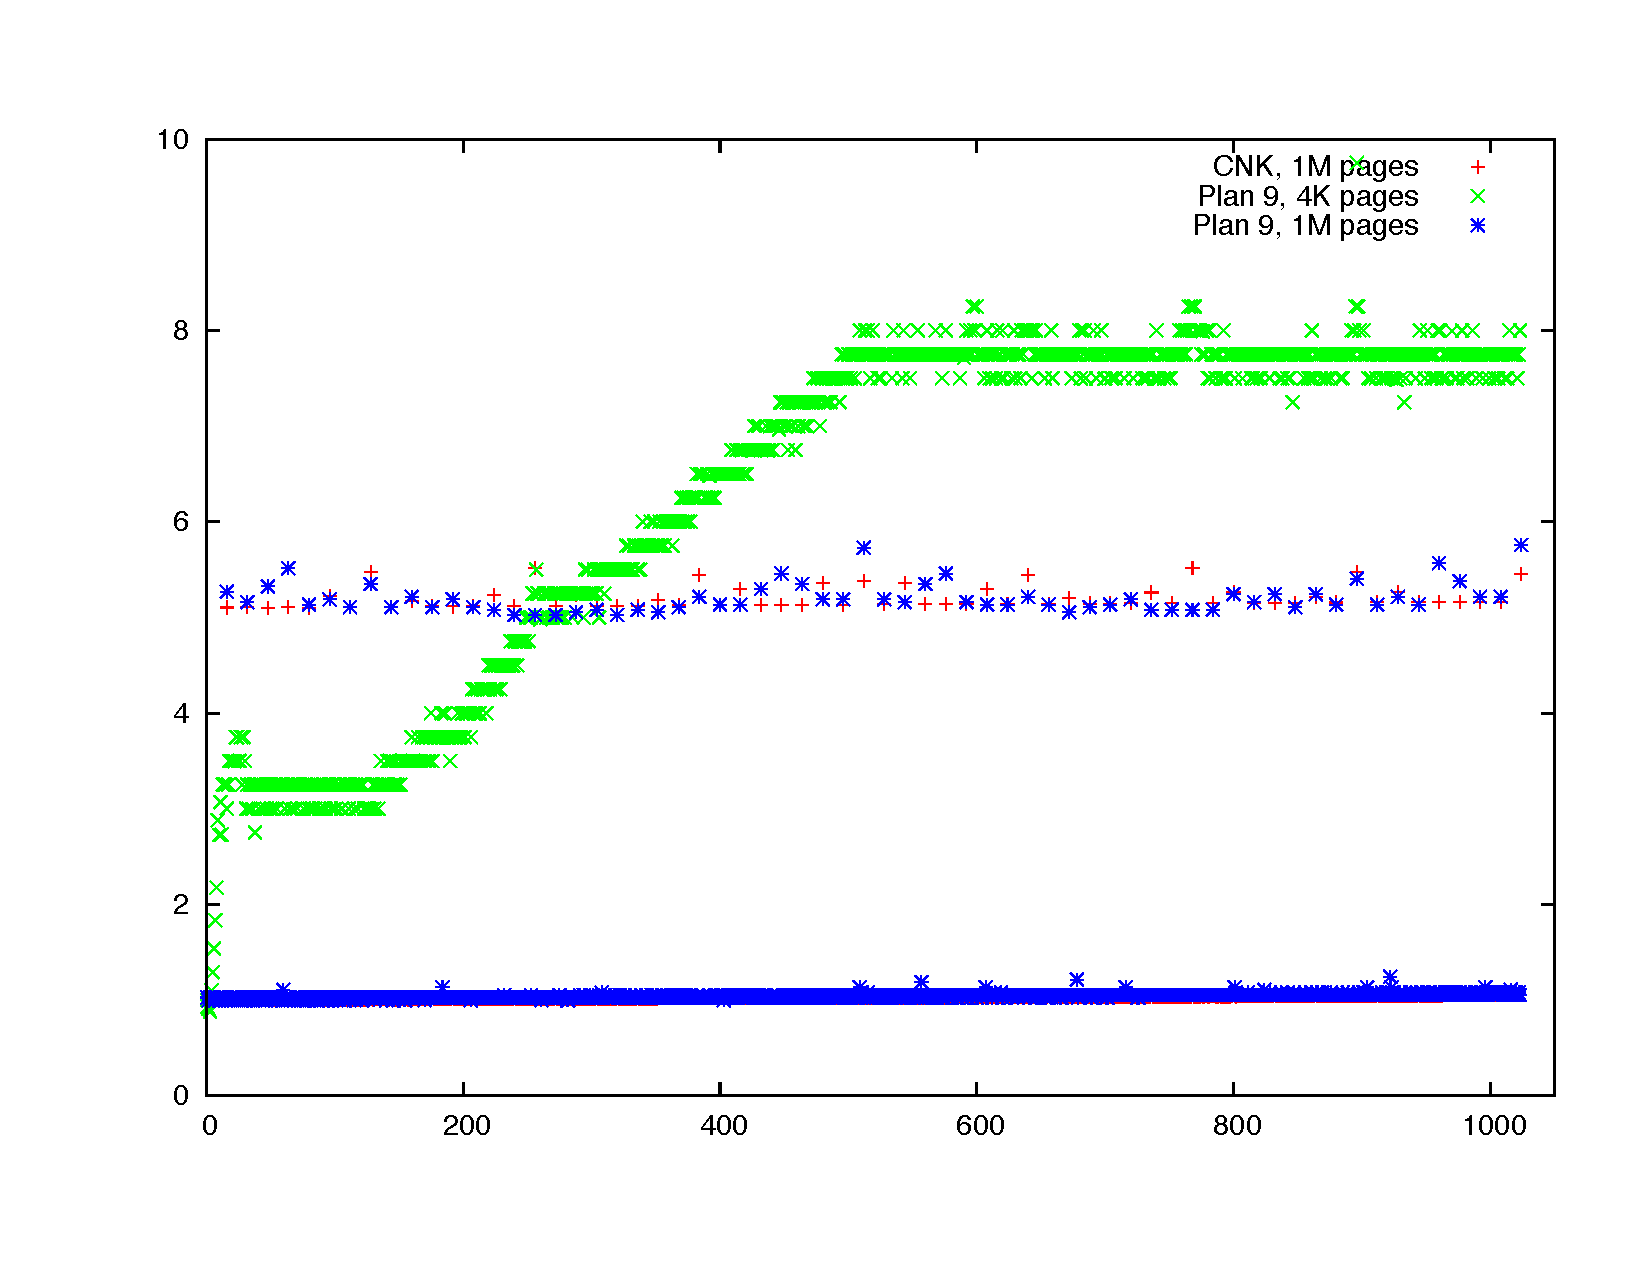
\includegraphics[width=4in]{strid3.pdf}
 \caption{{\bf Result of running strid3 on CNK, Plan 9, and Plan 9 with 1 MByte pages. }}
\label{strid3}
\end{center}
\end{figure}
to show the impact of TLB size upon an application. Shown in Figure \ref{strid3} is the result. Plan~9 is 
eight times slower than the CNK when 4096 byte pages are used. With one Mbyte pages in Plan~9, its 
performance is identical to the CNK. 
The change to Plan~9 to support the larger pages amounted to less than 30 lines of code\cite{DBLP:journals/ife/MinnichM09}. 

\section{Currying and Process-private system calls}
Extensive measurement of the kernel, using the tool developed and described in \cite{plan9trace}, showed
that for read and write system calls a great deal of overhead was repeated for each iteration of the 
call. Two of the biggest overheads are validation of the file descriptor and the read/write pointer and 
length validation. We also found in most cases that the pointers are being reused for each call: it is extremely rare for these parameters to be wrong, yet programs pay the full overhead for checking them 
each time. For the Blue Gene global barrier device, the overhead for the system call was 3.529 microseconds. 

In \cite{currying} we describe the possible approaches to resolving this problem. We developed two 
several extensions to Plan~9 that allowed the kernel to Curry the arguments to the read and write
system calls. The result: the file descriptor and point/length information is checked once, and the
result stored in a cache held in the proc struct (per-process information) in the kernel. The per-process structure is 
also extended with a private system call table. When the process makes a private system
call, all the standard checking is skipped and the cached values are used instead. This 
new system call path resulted in a 5-fold reduction in overhead, to 729 nanoseconds. 

The Currying and per-process system calls together form a new type of interface to operating system
kernels. 

\subsection{Shared Heap}
\section{File Systems}
\subsection{Compute Node Caches}
\section{New network communications models}
\subsection{Active Message Support}
\subsection{What are we calling Charles stuff?}
\section{Kittyhawk Kernels and VMM}

Supercomputers and clouds both strive to make a large number of 
computing cores available for computation. 
However, current cloud infrastructure does not yield the performance 
sought by many scientific applications. A source of the performance 
loss comes from virtualization and virtualization of the network in 
particular. 
Project Kittyhawk~\cite{kh-sciencecloud} was an undertaking at IBM Research 
to explore the use of a hybrid supercomputer software infrastructure
on top of a BlueGene/P which allows direct hardware access to the 
communication hardware for the necessary components while providing 
the standard elastic cloud infrastructure for other components.

Beyond the enabling infrastructure for cloud provisioning and dynamic
boot of multiple images across compute nodes within a single BG/P
allocation, the Kittyhawk team also ported a Linux compute node
implementation complete with an Ethernet interface to the high-performance
collective and torus networks~\cite{kh-systemsjournal}.  
This allowed Linux applications to run unmodified om Blue Gene compute 
nodes without incurring the performance 
overhead of reflecting sockets and I/O operations thorugh user space
helpers as in ZeptoOS.  It also enabled more conventional storage solutions
including SAN and NAS to be extended into the compute node network for
I/O intensive solutions.  While the Kittyhawk Linux kernel provided this
Ethernet interface, it also provided an API allowing the allocation of
torus channels directly to high performance applications which knew how to
interact with them allowing even greater degrees of performance and flexibility.
These allocated application channels co-existed with the kernel-space channels
providing a good hybrid trade off between system provided networking and
OS bypass.

The Kittyhawk environment was not limited to Linux kernel targets.  
It also supported execution of the L4 microkernel operating system.  
In addition to providing an alternative execution platform for applications,
the L4 Kittyhawk port also supported a virtual machine monitor which could
be used to further virtualize the BG/P nodes and network providing additional
protection in cloud deployment environments.

The Kittyhawk infrastructure, the linux kernel patches, and the L4 kernel
and virtual machine monitor have all been released as open source and are
available from http://kittyhawk.bu.edu.
